\section{Dataset} 
We collected the latest release (September, 2017) of Stack Exchange dataset. This snapshot is a complete archive of all activities in all Stack Exchange. 

There are 170 sites in our collected dataset. For the purpose of empirical analysis, we only consider the sites that have been active for at least 12 months beyond the ramp up period (site created, but few or no activity). There are 157 such sites. The age of these sites vary from 14 months to 111 months, number of user from 1072 to 547175, number of posts (questions and answers) from 1600 to 1985869. In addition, the sites have small overlaps in terms of user base, ranging from 0.1\% to 12\%. Therefore, we can reasonably argue that the underlying markets are independent. 

In Figure~\ref{fig:dataset} we present letter value plots to show the distribution of number of users, number of posts, and age for the Stack Exchange markets. Letter value plots include detailed information about the tails of the distribution, which is appropriate for large dataset such as ours. 


\iffalse
\begin{wrapfigure}{R}{0.2\textwidth}
\centering
\vspace{-\baselineskip}
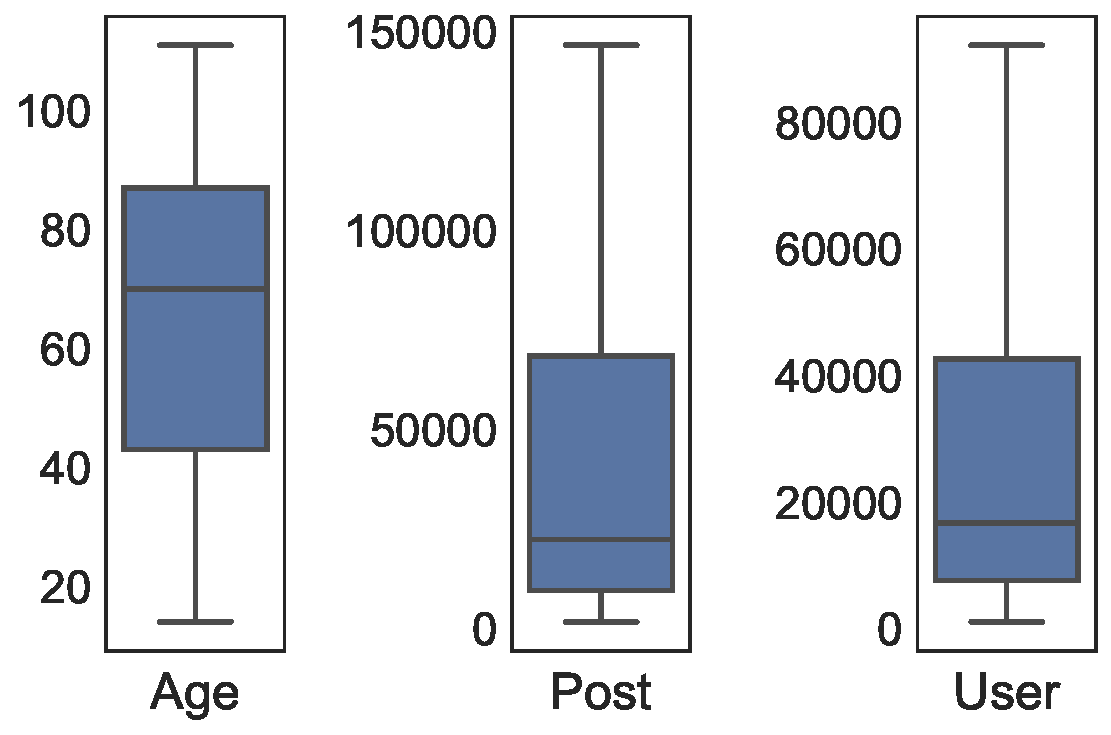
\includegraphics[width=0.2\textwidth]{Figures/Dataset_Statistics.pdf}
\caption{Site Statistics}
\vspace{-\baselineskip}
\end{wrapfigure}
\fi

\begin{figure}[hbt]
\centering
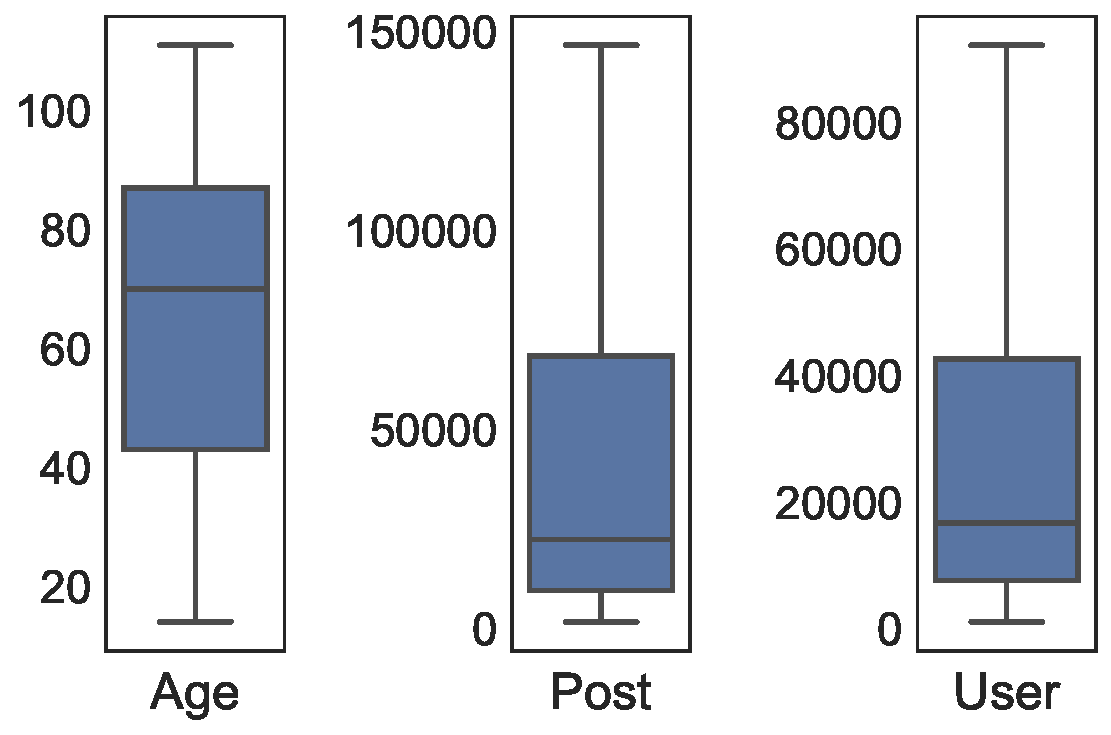
\includegraphics[scale=0.45]{Figures/Dataset_Statistics.pdf}
\caption{Distribution of number of users, number of posts, and age for Stack Exchange markets. The markets vary a lot in all three dimensions (users, activity, and age), as manifested by the letter value plots. }
\label{fig:dataset}
\end{figure}
